\chapter{Matching and Assignment Problems}

Hearing footsteps behind them, Ajur and Jura turned and saw Rishnak rushing to catch up with them.

Rishnak wasted no time and said, ``The edges analogue of a maximal independent set, which remember is a set of non-adjacent vertices, is called a \textit{maximal matching}. A maximal matching is a set of edges that do not share any common end vertices. Here is an example with maximal matching edges shown in red.''

Rishnak flashed his hands and a new graph appeared in front of Ajur [Figure~\ref{16g1}], four of its edges glimmering in red.

\begin{figure}
\begin{center}

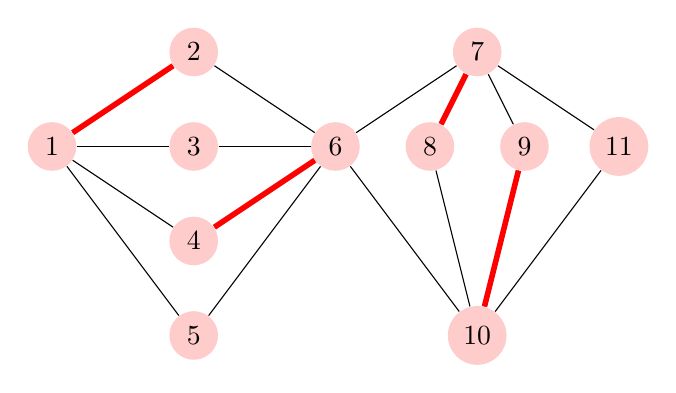
\begin{tikzpicture}
  [scale=.6,auto=left,every node/.style={circle,fill=red!20}]
  \node (n1) at (-1,1) {1};
  \node (n2) at (2,3)  {2};
  \node (n3) at (2,1)  {3};
  \node (n4) at (2,-1) {4};
  \node (n5) at (2, -3) {5};
  \node (n6) at (5,1)  {6};
  \node (n7) at (8,3)  {7};
  \node (n8) at (7,1) {8};
  \node (n9) at (9,1)  {9};
  \node (n10) at (8,-3)  {10};
  \node (n11) at (11,1) {11};

  \foreach \from/\to in {n1/n2,n1/n3,n1/n4,n1/n5,n2/n6,n3/n6/n4,n4/n6,n5/n6,n6/n7,n6/n10,n7/n8,n7/n9,n7/n11,
  n8/n10,n9/n10,n10/n11}
    \draw (\from) -- (\to);
\draw[-,line width=2 pt,red]
  (n1) to (n2);
  \draw[-,line width=2 pt,red]
  (n4) to (n6);
  \draw[-,line width=2 pt,red]
  (n7) to (n8);
  \draw[-,line width=2 pt,red]
  (n9) to (n10);
  \end{tikzpicture}
\caption{A graph for which maximal matching edges are shown in red}\label{16g1}
\end{center}
\end{figure}

Rishnak continued, ``This is a maximal matching. Every edge is incident at one of the end vertices of the edges in the maximal set. Therefore, vertices~$\{1,2,4,6,7,8,9,10\}$ form a vertex cover.''

Ajur said, ``But that vertex cover is not the minimum vertex cover.''

Rishnak said, ``You are sharp today, Ajur. Right, the minimum vertex cover is~$\{1,6,7,10\}$. If we find a maximal matching, we at least know the upper bound on the size of the minimum vertex cover for that graph.''

Ajur nodded.

Rishnak said, ``A \textit{perfect matching} is a maximal matching in which all of the vertices are the end vertices of the edges in the matching. For example, the graph already in front of you [Figure~\ref{16g1}] does not have a perfect matching, but this graph''---Rishnak waved his hands a new graph appeared [Figure~\ref{16g2}]---``does have a perfect matching since all of the vertices in the graph are end vertices of the edges in the perfect matching.''

\begin{figure}
\begin{center}
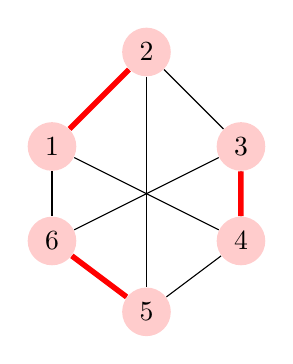
\begin{tikzpicture}
  [scale=.3,auto=left,every node/.style={circle,fill=red!20}]
  \node (n1) at (1,7) {1};
  \node (n2) at (5,11)  {2};
  \node (n3) at (9,7)  {3};
  \node (n4) at (9,3) {4};
  \node (n5) at (5,0)  {5};
  \node (n6) at (1,3) {6};
  
   \foreach \from/\to in {n1/n2,n2/n3,n3/n4,n4/n5,n5/n6,n1/n6,
  n2/n5, n6/n3,n1/n4}
    \draw (\from) -- (\to);
     \foreach \from/\to in {n1/n2,n5/n6,n3/n4}
    \draw[line width=2 pt,red] (\from) -- (\to);
    \end{tikzpicture}
\caption{A graph with a perfect matching with edges of the perfect matching shown in red}\label{16g2}
\end{center}
\end{figure}

Rishnak smiled as he went on. He said, ``Here is an interesting problem related to matching that actually earned Professors Lloyd Shapley and Alvin Roth the Nobel prize in Economics in 2012.  First, in the 1960s, Professors David Gale and Shapely introduced a problem called the stable marriage problem, which I will describe in a moment. Professor Roth applied this to a variety of applications, earning them the Nobel.''

Ajur raised his eyebrows, eager to hear more.

Rishnak said, ``The stable marriage problem may be stated as follows. Given~$n$ males and~$n$ females and a list of preferences for each male and female as to whom they would like to marry, we want to find stable marriages for everyone in the entire group.
A marriage is unstable if there is a pair of individuals who are not married to one another but prefer one another over their respective spouses. Otherwise, the marriage is stable.''

Ajur rolled his eyes and said, ``Wow, what a weird problem.''

Rishnak continued, ``Okay, let us consider the preferences for males in this table''---he flashed his hands and showed a table of data [Table~\ref{16t1}]---``and for females in this table''---with a wave of his hand, Rishnak produced a second table [Table~\ref{16t2}].

\begin{table}
\begin{center}
\begin{tabular}{ |p{3cm}||p{1.5cm}||p{1.5cm} || p{1.5cm}|| }
 \hline
 \hline
 Male Name & First&Second&Third\\
 \hline
 Al  & Carla    &Ada&Bea\\
Bob&Ada&Bea&Carla\\
Caleb&Ada&Carla&Bea\\
 
 
 \hline
\end{tabular}
\caption{Male preferences in the stable marriage problem}\label{16t1}
\end{center}
\end{table}
\begin{table}
\begin{center}
\begin{tabular}{ |p{3cm}||p{1.5cm}||p{1.5cm} || p{1.5cm}|| }
 \hline
 \hline
 Female Name & First&Second&Third\\
 \hline
 Ada  & Al    &Bob&Caleb\\
Bea&Caleb&Al&Bob\\
Carla&Al&Caleb&Bob\\
 
 
 \hline
\end{tabular}
\caption{Female preferences in the stable marriage problem}\label{16t2}
\end{center}
\end{table}

Rishnak said, ``Given these preferences, we can determine that the following marriages are stable:~(Al, Carla), (Bob, Ada), and (Caleb, Bea). We know this because there are no unstable pairs; however, marriages (Al, Carla), (Bob, Bea), and (Caleb, Ada) are unstable marriages since Bob prefers Ada over Bea and Ada prefers Bob over Caleb.''

Ajur said, ``I see.''

Rishnak continued, ``Gale and Shapley showed that there is always a stable marriage pair for any set of preferences.''

Ajur raised his eyebrows again.  He asked, ``How?''

Rishnak said, ``The algorithm they developed is rather elegant. Here it is:

\begin{enumerate}
    \item In the first round, each male proposes to the female he prefers the most.
    \item Each female replies with a `maybe' to the suitor she most prefers and a `no' to all other suitors. She is temporarily engaged to the male she most prefers thus far.
    \item In the subsequent round, each non-engaged male proposes to the most-preferred female\footnote{Each male starts from his most preferred female and proceeds through to his least preferred female.} to whom he has not yet proposed, regardless of whether this female is already engaged.
    \item Each female replies `maybe' if she is currently not engaged or if she prefers this male over her current provisional partner. In this case, she rejects her current provisional partner who then becomes non-engaged. The provisional nature of engagements preserves the right of an already engaged female to essentially trade up and, in the process, jilt her until-then partner.
   \item We repeat Steps~3 and 4 until everyone is engaged.''
\end{enumerate}

Ajur frowned as this was a lot to understand. He decided to apply this procedure to the data still in front of him [Table~\ref{16t1}] [Table~\ref{16t2}]. He said, ``Okay, after the first round, Al is temporarily engaged to Carla and Bob is temporarily engaged to Ada since both Bob and Caleb opt for Ada, but Ada prefers Bob over Caleb. In the next round, Caleb proposes to Carla, who is temporarily engaged to Al. Since Carla prefers Al over Caleb, Caleb's offer is rejected. Next, Caleb proposes to Bea, his last choice, and Bea accepts Caleb since she does not have a suitor thus far. Then the algorithm terminates with the stable marriage pairs of (Al, Carla), (Bob, Ada), and (Caleb, Bea).''

Rishnak smiled and said, ``Precisely.''

Ajur said, ``This algorithm sounds like a messy game of musical chairs.''

Rishnak laughed and said, ``Another application of the matching problem is the optimal assignment problem. Here, we need to assign jobs to a group of workers, with the cost required for each worker to do each job as a given. We wish to find an assignment of workers to jobs so as to minimize the total cost.''

Ajur thought of one of his favorite types of graphs. He said, ``We can use a bipartite graph with workers in one partition and jobs in the other partition.''

Rishnak said, ``Yes, an edge from worker~$i$ to job~$j$ has the cost of worker~$i$ doing job~$j$.
Let us assume that the number of workers is equal to the number of jobs---this can be~$n$.''

Rishnak flashed his hands and a new table of data appeared in front of Ajur [Table~\ref{16t3}]. Rishnak said, ``Here is a cost matrix showing how much each job would cost for our three workers, Al, Bob, and Caleb.''

\begin{table}
\begin{center}
\begin{tabular}{ ||p{2cm}||p{2cm}||p{1.5cm} ||p{1.5cm}|| }
 \hline
 
  & Salesman&Tutor&Chef\\
 \hline
 Al  & 17   &40&45\\
 Bob& 23&60&35\\
 Caleb&21&40&25\\

 
 \hline
\end{tabular}
\caption{Cost matrix in which rows represent workers and columns represent the jobs they can do; the numeric values show the cost for each worker to do each job}\label{16t3}
\end{center}
\end{table}

Ajur studied the data.

Rishnak said, ``For the optimal assignment problem, we want to assign jobs to minimize the total overall cost. Here is an algorithm we can use:

\begin{enumerate}
\item For each row of the matrix, circle the smallest element and subtract that from every other element in the same row.
\item Also perform Step~1 for all of the columns.
\item Cover all zeros in the matrix using a minimum number of horizontal and vertical lines. In other words, cross these zeros out, which might also cover non-zero values.
\item If the minimum number of lines we draw in Step~3 is~$n$, an optimal assignment is possible and we are done. Otherwise, proceed to Step~5.
\item Determine the smallest entry not yet covered by any line. Subtract this entry from each uncovered row, then add it to each covered column. Next, erase all of the lines and return to Step~3 to perform the crossing out step again.''
\end{enumerate}

Ajur again studied the data. He said, ``Let me try this out. And~$n=3$ for this problem.'' He copied the table in the dirt and performed the first step, subtracting the smallest element from every other element in the same row [Table~\ref{16t4}].
Ajur quickly went on to Step~2, subtracting out the smallest value in each column [Table~\ref{16t5}].

\begin{table}
\begin{center}
  \begin{tikzpicture}
    \matrix (M)[matrix of math nodes,left delimiter={[},right delimiter={]}]{
     0&23&28\\
     0&37&12\\
     0&19&4\\
     };
     %\draw[thick,black](M-1-1.west)--(M-1-4.east);
     %\draw[thick,black](M-1-1.north)--(M-4-1.south);
     %\draw[thick,black](M-1-3.north)--(M-4-3.south);
  \end{tikzpicture}

\caption{The table for the optimal assignment problem after Step~1}\label{16t4}
\end{center}
\end{table}

\begin{table}
\begin{center}
  \begin{tikzpicture}
    \matrix (M)[matrix of math nodes,left delimiter={[},right delimiter={]}]{
     0&4&24\\
     0&18&8\\
     0&0&0\\
     };
     %\draw[thick,black](M-1-1.west)--(M-1-4.east);
     %\draw[thick,black](M-1-1.north)--(M-4-1.south);
     %\draw[thick,black](M-1-3.north)--(M-4-3.south);
  \end{tikzpicture}

\caption{The table for the optimal assignment problem after Step~2}\label{16t5}
\end{center}
\end{table}

Ajur said, ``Okay, let me now cross out the zeros in as few horizontal and vertical lines as possible.'' He drew two lines [Table~\ref{16t6}].

\begin{table}
\begin{center}
  \begin{tikzpicture}
    \matrix (M)[matrix of math nodes,left delimiter={[},right delimiter={]}]{
     0&4&24\\
     0&18&8\\
     0&0&0\\
     };
     \draw[thick,black](M-3-1.west)--(M-3-3.east);
     \draw[thick,black](M-1-1.north)--(M-3-1.south);
     %\draw[thick,black](M-1-3.north)--(M-4-3.south);
  \end{tikzpicture}

\caption{The table for the optimal assignment problem after Step~3}\label{16t6}
\end{center}
\end{table}

Ajur frowned and said, ``Since there are two lines and~$n=3$, we go from Step~4 to Step~5, taking the smallest entry from among the uncovered entries---so that would be~4---and subtracting it from each uncovered row.'' Ajur scribbled in the dirt, updating the first two rows [Table~\ref{16t7}].

He said, ``Wait, now I need to also add it to each covered column''---he did so [Table~\ref{16t8}]---``and erase all of the lines, then go back to Step~3.''

\begin{table}
\begin{center}
  \begin{tikzpicture}
    \matrix (M)[matrix of math nodes,left delimiter={[},right delimiter={]}]{
     -4&0&20\\
     -4&14&4\\
     0&0&0\\
     };
     \draw[thick,black](M-3-1.west)--(M-3-3.east);
     \draw[thick,black](M-1-1.north)--(M-3-1.south);
     %\draw[thick,black](M-1-3.north)--(M-4-3.south);
  \end{tikzpicture}

\caption{The table for the optimal assignment problem after the subtraction in Step~5}\label{16t7}
\end{center}
\end{table}
\begin{table}
\begin{center}
  \begin{tikzpicture}
    \matrix (M)[matrix of math nodes,left delimiter={[},right delimiter={]}]{
     0&0&20\\
     0&14&4\\
     4&0&0\\
     };
     \draw[thick,black](M-3-1.west)--(M-3-3.east);
     \draw[thick,black](M-1-1.north)--(M-3-1.south);
     %\draw[thick,black](M-1-3.north)--(M-3-3.south);
     %\draw[thick,black](M-1-1.north)--(M-3-1.south);
     %\draw[thick,black](M-1-2.north)--(M-3-2.south);
  \end{tikzpicture}

\caption{The table for the optimal assignment problem after Step~5}\label{16t8}
\end{center}
\end{table}

Ajur drew three vertical lines [Table~\ref{16t9}]. He said, ``Now we have exactly three lines covering all of the zeros, so we are done. Ignoring the lines, we can find the assignments to be Caleb as Chef, Al as Tutor, and Bob as Salesman. This gives us a total cost of~$25+40+23=88$.''

\begin{table}
\begin{center}
  \begin{tikzpicture}
    \matrix (M)[matrix of math nodes,left delimiter={[},right delimiter={]}]{
     0&0&20\\
     0&14&4\\
     4&0&0\\
     };
     %\draw[thick,black](M-3-1.west)--(M-3-3.east);
     %\draw[thick,black](M-1-1.north)--(M-3-1.south);
     \draw[thick,black](M-1-3.north)--(M-3-3.south);
     \draw[thick,black](M-1-1.north)--(M-3-1.south);
     \draw[thick,black](M-1-2.north)--(M-3-2.south);
  \end{tikzpicture}

\caption{The table for the optimal assignment problem after Step~4 in which the algorithm stops}\label{16t9}
\end{center}
\end{table}

Rishnak said, ``Good, Ajur.''

Ajur said, ``But how is this problem related to the perfect matching problem?''

Rishnak was patient and explained the relation between these two problems. He said, ``The jobs and workers can be thought of as vertices of a bipartite graph, with one set of vertices being the workers and the other set being the jobs. If we assume that both sets of vertices have the same size, we can
construct a complete bipartite graph, meaning there is an edge from every worker to every job. Remember that if a job~$j$ has cost~$w$ for worker~$i$, then the corresponding edge~$(i,j)$ gets assigned a weight of~$w$.''

Ajur followed Rishnak so far.

Rishnak continued, ``For example, the table still in front of you [Table~\ref{16t3}] can be represented by this complete weighted bipartite graph.'' Rishnak flashed his hands and a new graph appeared [Figure~\ref{16g3}].

Ajur studied the graph, seeing how it related to Table~\ref{16t3}]. He said, ``And the perfect matching problem applies to this graph then?''

Rishnak said, ``Yes, to solve the optimal assignment problem, we can simply find the minimum perfect matching in this bipartite graph representation.''

Ajur smiled, satisfied that all of these problems had interesting connections.

\begin{figure}
\begin{center}

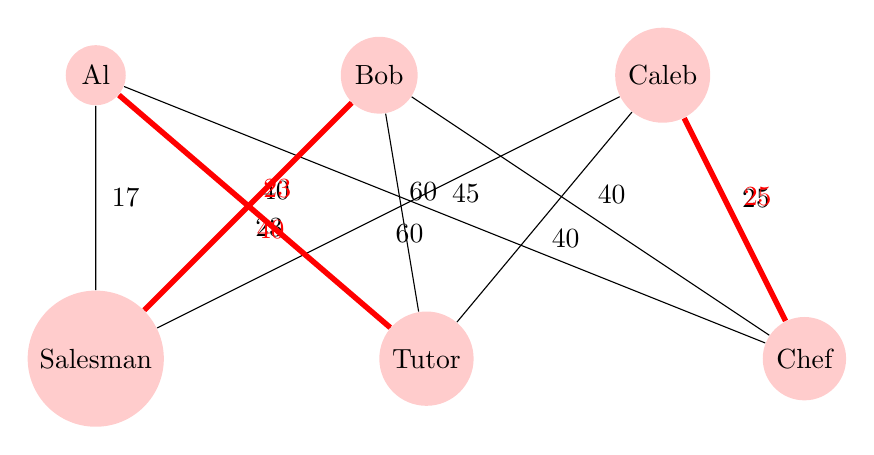
\begin{tikzpicture}
  [scale=.6,auto=left,every node/.style={circle,fill=red!20}]
  \tikzstyle{weight} = [fill=none]
  \node (n1) at (-1,5) {Al};
  \node (n2) at (5,5)  {Bob};
  \node (n3) at (11,5)  {Caleb};
  \node (n4) at (-1,-1) {Salesman};
  \node (n5) at (6, -1) {Tutor};
  \node (n6) at (14,-1)  {Chef};
 
\foreach \source /\dest /\weight in {n1/n4/17,n1/n5/40,n1/n6/45}       %%%%%%% need to fix this
   \draw (\source) --node[weight] {$\weight$}  (\dest);
\foreach \source /\dest /\weight in {n2/n4/23,n2/n5/60,n2/n6/40} 
   \draw (\source) --node[weight] {$\weight$}  (\dest);
\foreach \source /\dest /\weight in {n3/n4/60,n3/n5/40,n3/n6/25} 
   \draw (\source) --node[weight] {$\weight$}  (\dest);
\foreach \source /\dest /\weight in {n2/n4/40,n1/n5/23,n3/n6/25} 
   \draw[color=red,line width=2 pt] (\source) --node[weight] {$\weight$}  (\dest); 
 
  \end{tikzpicture}
\caption{Complete bipartite graph corresponding to Table~\ref{16t3} with weights representing the costs and the minimum perfect matching edges shown in red}\label{16g3}
\end{center}
\end{figure}

\begin{newpage}
\end{newpage}

\subsection*{Question for the fourteenth day}
Seeing Ajur was tired, Rishnak said, ``Here we are, Ajur, ready for the questions for the fourteenth day.'' Rishnak flashed his hands and two tables appeared [Table~\ref{16tq1}] [Table~\ref{16tq2}].

Rishnak said, ``These two tables show the preferences for males and females. Assume already that~$M2$ and~$W1$ are temporarily engaged. If~$M3$ approached~$W1$ with a proposal, what would~$W1$ do? Next, flipping this around, assume~$W1$ is married to~$M2$. Who would~$W2$ approach then?''

\begin{table}
\begin{center}
\begin{tabular}{ |p{3cm}||p{1.5cm}||p{1.5cm} || p{1.5cm}|| }
 \hline
 \hline
 Male Name & First&Second&Third\\
 \hline
 M1  & W1   &W3&W2\\
 M2&W3&W2&W1\\
M3&W3&W1&W2\\
 
 
 \hline
\end{tabular}
\caption{Male preferences}\label{16tq1}
\end{center}
\end{table}

\begin{table}
\begin{center}
\begin{tabular}{ |p{3cm}||p{1.5cm}||p{1.5cm} || p{1.5cm}|| }
 \hline
 \hline
 Female Name & First&Second&Third\\
 \hline
 W1 & M2    &M1&M3\\
W2&M2&M3&M1\\
W3&M1&M2&M3\\
 
 
 \hline
\end{tabular}
\caption{Female preferences}\label{16tq2}
\end{center}
\end{table}

\textit{Before you turn the page, try to come up with answers of your own!}

\newpage
\subsection*{Answer for the fourteenth day}
Ajur studied the data and walked through Rishnak's questions in his head. At length, he said, ``$W1$ will reject the proposal from~$M3$ since~$W1$ prefers~$M2$ over~$M3$. And if women are proposing,~$W2$ will approach~$M2$ first.''

Rishnak nodded.

Ajur was deep in thought, more interested in why and how these procedures work.

Seeing Ajur's puzzled look, Rishnak said, ``Do not fret, Ajur. I myself had not understood these things very well, but you will learn this all in college.''

This seemed to be okay with Ajur. He nodded and left with Jura.
